\documentclass[12pt]{report}

\usepackage[utf8]{inputenc}
\usepackage{graphicx}
\usepackage{amssymb}
\usepackage{amsmath}
\usepackage{amsthm}
\usepackage{hyperref}
\usepackage[super]{natbib}
\bibliographystyle{unsrtnat}

\graphicspath{ {images/} }

\theoremstyle{definition}
\newtheorem{example}{Example}[section]
\newtheorem{definition}{Definition}[section]
\newtheorem{theorem}{Theorem}[section]
\newtheorem{notation}{Notation}[section]

\title 
{
	{KMS states and Tomita-Takesaki Theory}\\
	{\large Universidad de los Andes}\\
	{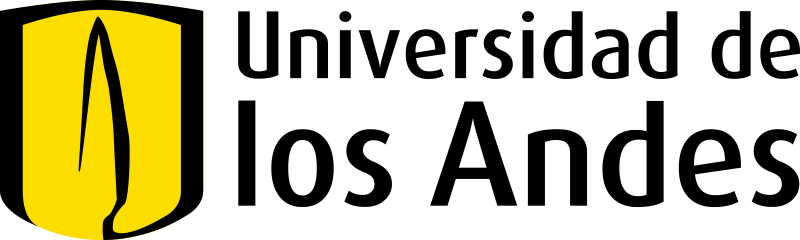
\includegraphics{logo.png}}	
}
\author{Iván Mauricio Burbano Aldana}

\begin{document}

\maketitle

\tableofcontents

\chapter{Introduction}

\chapter{Classical and Quantum Mechanics as Probability Theories}
This chapter shows how both classical and quantum mechanics are probability theories. This is not intended as an axiomatization of these theories. Indeed the reader is assumed to be comfortable with these physical theories as well as the basic mathematical concepts of measure theory and functional analysis.

\section{Classical Mechanics}\label{sec:classical_probability}

The setting of classical mechanics is usually a locally compact Hausdorff space $X$. We consider the states of maximal knowledge (or pure states) to be the elements of $X$. Likewise, observables take the form of functions on $X$. We call the points of $X$ states of maximal knowledge because we interpret $f(p)$ as the value of the observable $f$ in the state $p\in X$. Moreover, given that in principle we could make the value of an observable as precise as we want by improving our knowledge of the state, observables are elements of the set of continuous functions $C(X)$\footnote{It doesn't matter whether we consider them real or complex at this stage.}. Nonetheless the purpose of statistical mechanics is to treat systems in which total knowledge of a state is not practically possible. Instead we consider a probability measure\footnote{Along with a $\sigma$-algebra which we won't mention explicitly to keep the notation simple but should always be kept in mind.} which assigns to every measurable subset of $X$ a probability of the system's state being in it. We may define the expected value of an observable $f\in C(X)$ through a probability measure $P$ by 
\begin{equation}\label{eq:classical_states}
\langle f \rangle_P = \int fdP.
\end{equation}  
Notice that an element $p\in X$ can also be though as a probability measure by using the Dirac measure $\delta_p$ which assigns $1$ to a set if it contains $p$ and $0$ otherwise. Indeed for every element $p \in X$ and observable $f \in C(X)$ we have $\langle f \rangle_{\delta_p} = f(p)$. This motivates us to broaden the definition of states to the probability measures on $X$. We will call Dirac measures (or equivalently the points in $X$) pure states.

This definition of state proves to be very helpful for the discussion of ensembles. Whenever the description of the state of a system as a pure state is not feasible, we may consider the set of outcomes $Y$ of measurements we may perform on the system. Every element of $Y$ gives us information of the system in the form of a finite measure. We may define an ensemble as the mapping from $Y$ into the set of finite measures on $X$. Through normalization of finite measures every ensemble yields a mapping from $Y$ into the set of states and we define the accessible (pure) states of an element $y\in Y$ to be the support of the corresponding state. Although the construction of an ensemble is in general a difficult task, for systems in statistical equilibrium\footnote{These are systems whose state does not change in time. We refer to the equilibrium as statistical because it may be that the pure state of the system is changing in time but noticing these changes is not feasible for us.} there are many standard procedures. In the case of these type of systems we define the partition function $Z:Y\to \mathbb{R}^+_0$ by assigning to every element $y$ the measure of $X$ given by the ensemble evaluated at $y$.

\begin{example}
In many physical systems the space of pure states has a natural notion of size which we may represent by giving it the structure of a measure space $(X,\mathcal{A},\mu)$ where $\mathcal{A}$ contains the Borel $\sigma$-algebra\footnote{Usually we take a countable set with the counting measure but another example would be a phase space with the Liouville measure. In the latter, it is common that $H^{-1}(y)$ is a set of measure zero so we actually have to take $X=H^{-1}(y)$ with the appropriate induced measure.} . We may consider $Y = \mathbb{R}$ to be the set of energy outcomes. If $H:X\rightarrow \mathbb{R}$ is a measurable function taking the interpretation of energy we define the microcanonical ensemble to be the mapping $y\mapsto \mu_y$ where $\mu_y(\Sigma) = \mu(\Sigma\cap H^{-1}(y))$ for all measurable $\Sigma$. The set $H^{-1}(y)$ is the set of accessible states and $\mu_y(\Sigma)$ measures the amount of pure states in $\Sigma$ which are accessible. Notice that the normalization of $\mu_y$ yields a state $P_y$ which assigns a uniform probability measure to $X$. This is called the equal a priori probabilities postulate. In this ensemble the partition function $Z(y) = \mu_y(X) = \mu(H^{-1}(y))$ is just the amount of accessible states. This ensemble is usually used to describe systems with constant energy and a fixed number of particles.
\end{example}

\begin{example}
Consider again a measure space $(X,\mathcal{A},\mu)$ but let $Y=\mathbb{R}^+$ be the set of inverse temperatures of the system. If we have an energy function $H:X\rightarrow \mathbb{R}$ such that $x\rightarrow \exp(-y H(x))$ is integrable for all $y \in Y$ the canonical ensemble assigns to every inverse temperature $y$ a finite measure $\mu_y$ by
\begin{equation}
\mu_y(\Sigma)=\int_\Sigma e^{-y H(x)}d\mu(x)
\end{equation}
for all measurable sets $\Sigma$. This ensemble is usually used to describe systems with a fixed number of particles in thermal equilibrium with a heat bath. Note that we could add to the description of the system the heat bath and we would be able to in principle use the microcanonical ensemble. The difficulty lies in that generally the counting of accessible states is more difficult than the application of the canonical ensemble.
\end{example}

Note that both of the ensembles discussed have images consisting of absolutely continuous measures $\mu_y$ with respect to the notion of size $\mu$. The same is true for the induced states $P_y$. Moreover the Lebesgue-Radon-Nikodým derivative exits and we define the entropy of the ensemble in the state $P_y$ by\footnote{In general if we start from a decomposable $(X,\mathcal{A},\mu)$ and have an ensemble which yields absolutely continuous measures with respect to $\mu$ we can define entropy in this fashion. In particular, if $\mu$ comes from the Daniel extension of a positive linear functional the space is decomposable.}
\begin{equation}
S(P_y)=-\int_{supp(P_y)} \log\left(\frac{dP_y}{d\mu}\right)dP_y=-\langle\log\left(\frac{dP_y}{d\mu}\right)\chi_{supp P_y}\rangle_{P_y}.
\end{equation}
One can check that in the microcanonical ensemble 
\begin{equation}
\frac{dP_y}{d\mu}(x)=\frac{\chi_{H^{-1}(y)}(x)}{Z(y)}
\end{equation}
and in the canonical ensemble 
\begin{equation}
\frac{dP_y}{d\mu}(x)=\frac{\exp(-yH(x))}{Z(y)}. 
\end{equation}
In the case we have a state of maximal knowledge $\delta_p$ we may collapse $X$ to $(\{p\},\{\{p\},\emptyset\},\delta_p)$ and define an ensemble $y\mapsto \delta_p$. Such an ensemble has zero entropy.

\section{Quantum Mechanics}\label{sec:QM}

The setting of quantum mechanics is a separable Hilbert space $\mathcal{H}$. In this case the states are the non-negative self-adjoint operators of unit trace on $\mathcal{H}$ (called density operators) and observables take the form of self-adjoint operators on $\mathcal{H}$. The possible outcomes of an observable $A$ are the elements of its spectrum and, if $P_A$ is the unique projection-valued measure such that $A=\int id_\mathbb{R}dP_A$ given by the spectral theorem, we have that the probability of the measurement of the observable $A$ yielding a value in the measurable subset $E\subseteq\mathbb{R}$ in the state $\rho$ is $tr(P_A(E)\rho)$. One can check that given this way of measuring probabilities we have that the expected value of an observable $A$ in the state $\rho$ is
\begin{equation}\label{eq:quantum_states}
\langle A\rangle_\rho = tr(A\rho).
\end{equation}
Moreover we define the entropy of a state $\rho$ to be
\begin{equation}\label{eq:Q_entropy}
S(\rho)=-tr(\log(\rho)\rho)=-\langle log(\rho)\rangle_\rho.
\end{equation}
Inspired by the classical case we define a pure state $\rho_\psi$ to be orthogonal projection on the span of $\psi$ for $\psi\in\mathcal{H}$ of unit norm. Although such a state has null entropy as in the classical case
\begin{equation}\label{eqn:entropy_pure}
S(\rho_\psi)=-tr(\log(\rho_\psi)\rho_\psi)=-\langle\psi,\log(1)\psi\rangle = 0,
\end{equation} 
we can't in general associate to an observable $A$ a definite outcome unless $\psi$ is an eigenvector of $A$ corresponding to an eigenvalue $\lambda$ where we have 
\begin{equation}
tr(P_A(\{\lambda\})\rho_\psi)=\langle\psi,P_A(\{\lambda\})\psi\rangle=\langle\psi,\psi\rangle=\|\psi\|^2=1. 
\end{equation}
Notice that we haven't inspired the definition of a state like we did in the classical case. The connection between states and probability is given through the study of quantum logic in the next chapter.

\chapter{Quantum Probability}
The previous chapter showed that there is a dictionary to understand in a very similar language quantum and classical theories. Before we develop the language of operator algebras to make this similarity more concrete we will first show how this two theories are different. To do this we will study the logical structure of quantum mechanics and show that it isn't boolean.

\section{EPR paradox}

Einstein, Podolsky and Rosen examined the completeness of quantum mechanics in their famous 1935 paper \cite{Einstein1935}. They considered that an element of physical reality was one whose outcome in a measurement could be predicted without actually performing the experiment. They defined that a physical theory was complete if to every element of physical reality there corresponded an object in the theory. One can prove that in quantum mechanics two observables $A$ and $B$\footnote{We will assume them to be bounded to avoid technical difficulties since our example will be finite dimensional.} satisfy for every state $\rho$ the Heisenberg uncertainty relation
\begin{equation}
\Delta_\rho A\Delta_\rho B\geq\frac{1}{2}|\langle\left[A,B\right]\rangle_\rho|
\end{equation}
where $\left[A,B\right]=AB-BA$ is the commutator and $\Delta_\rho A=\sqrt{\langle A^2\rangle-\langle A\rangle^2}$. Therefore either quantum mechanics is incomplete or two non-commuting observables cannot have a simultaneous physical reality. Assuming that quantum mechanics is indeed complete we are forced to accept that two non-commuting observables don't have a simultaneous physical reality.

\begin{example}\label{ex:Bell}
To describe the polarization of a photon we may consider the Hilbert space $\mathbb{C}^2$. We assign to the proposition ``\textit{the photon is linearly polarized at an angle $\theta$ (1 means that this is the case and 0 that it isn't)}'' the operator $P(\theta)$ the orthogonal projection to the span of 
\begin{equation}
|\theta\rangle=\cos(\theta)(1,0)+\sin(\theta)(0,1).
\end{equation}
Therefore the vector $|\theta\rangle$ takes the interpretation the state in which the photon is certain to have linear polarization at angle $\theta$. Now consider a system with two photons in a state $\rho_{\psi}$ where 
\begin{equation}
\psi=\frac{1}{\sqrt{2}}\left(|0\rangle\otimes|\pi/2\rangle-|\pi/2\rangle\otimes|0\rangle\right).
\end{equation}
We may prepare such a system by allowing a Calcium atom to decay into two photons and waiting till the photons are far apart. It's easy to see that 
\begin{equation}
\psi=\frac{1}{\sqrt{2}}\left(|\pi/4\rangle\otimes|3\pi/4\rangle-|3\pi/4\rangle\otimes|\pi/4\rangle\right).
\end{equation}
Therefore if we measure that the first photon has horizontal polarization we know the second one has a vertical polarization and if we measure that the first one has a polarization at an angle $\pi/4$ we know the second one has an angle of $3\pi/4$. But since the photons are far apart, measurements on the first one cannot affect the second one. Therefore both states $|\pi/2\rangle$ and $|3\pi/4\rangle$ describe the same physical reality and we are forced to conclude that $P(\pi/2)$ and $P(3\pi/4)$ have simultaneous realities. Nonetheless since $|\pi/2\rangle$ is not orthogonal to $|3\pi/4\rangle$ the two projections don't commute arriving to a contradiction. 
\end{example}

Contradictions of the type shown above due to the use of coupled systems are often referred to nowadays as the EPR paradox. They led to the notion of entanglement. We are therefore, subject to the definitions given in the paper \cite{Einstein1935} forced to the conclusion that quantum theory must be an incomplete theory.  

\section{Lattices of Propositions and Bell's Inequalities}

We may continue EPR's agenda and try to find a complete theory of physical reality. In such a theory (much like in every physical theory) we must be able to ask true or false questions about a physical system. Studying these questions gives us an excuse to begin the discussion of logic theory. Although previous knowledge of logic is not essential, we will use our experience from classical logic to inspire the definitions we will use.

\begin{definition}
An order relation on a set $P$ is a relation $\leq$ on $X$ which satisfies for all $p,q,r\in P$:
\begin{itemize}
\item reflexivity: $p\leq p$;
\item antisymmetry: $p\leq q$ and $q\leq p$ implies $p=q$;
\item transitivity: $p\leq q$ and $q\leq r$ implies $p\leq r$.
\end{itemize}
The pair $(P,\leq)$ is called a partially ordered set or poset.
\end{definition}

We may recognize these laws if we exchange the symbols $\leq$ for the implication symbol $\implies$ as rules propositions evidently follow. Much like in this case, the rest of the definitions ahead will have a counterpart in propositional logic and are intended as an extension of it.   

\begin{definition}
Let $(P,\leq)$ be a poset and $A\subseteq P$. A lower (upper) bound of $A$ is an element $p\in P$ such that for all $a \in A$ we have $p\leq a$ ($a\leq p$). An infimum (supremum) of $A$ is a lower (upper) bound $p$ of $A$ such that if $r\in P$ is a lower (upper) bound of $A$ then $r\leq p$ ($p\leq r$).     
\end{definition}

Once again, through the symbol exchange made earlier we may note that the conjunction of two propositions $p\wedge q$ is the infimum of $\{p,q\}$ and the disjunction $p\vee q$ is the supremum of $\{p,q\}$. The infimum and sumpremum are closely related and we will in general carry the discussion only for the infimum leaving the details of the supremum in parenthesis just as we did in the previous definition. 

\begin{theorem}
Let $(P,\leq)$ be a poset and $A\subseteq P$ such that its infimum (supremum) exists. Then the infimum (supremum) is unique. 
\end{theorem}

\begin{proof}
Suppose $p$ and $q$ are infima (suprema) of $A$. Then since $p$ is a lower (upper) bound we have $p\leq q$ ($q\leq p$). Similarly, since $q$ is a lower (upper) bound $q\leq p$ ($p\leq q$). Therefore by antisymmetry $p=q$.  
\end{proof}

\begin{notation}
Let $(P,\leq)$ be a poset and $A\subseteq P$ such that its infimum (supremum) exists. We denote the infimum (supremum) of $A$ by $\bigwedge A$ ($\bigvee A$). If $A=\{p,q\}$ then we denote $p\wedge q :=\bigwedge A$ ($p\vee q := \bigvee A$). As is common in logic literature we will now use for infimum (supremum) the term meet (join). 
\end{notation}

Now we shall list some of the algebraic properties of posets.

\begin{theorem}\label{thm:logic_algebra}
Let $(P,\leq)$ be a poset. Then for all $p,q,r\in P$:
\begin{enumerate}
\item $p\leq q$ if and only if $p=p\wedge q$ if and only if $q =p\vee q$;
\item (idempotency) $p\wedge p = p$ and $p\vee p=p$;
\item (associativity) if the meet (join) of $\{p,q\}$, $\{q,r\}$, $\{p\wedge q, r\}$ ($\{p\vee q, r\}$), $\{p,q\wedge r\}$ ($\{p,q\vee r\}$) and $\{p,q,r\}$ exists then $(p\wedge q)\wedge r=p\wedge(q\wedge r)=\bigwedge \{p, q, r\}$ ($(p\vee q)\vee r=p\vee(q\vee r)=\bigvee \{p, q, r\}$);
\item (commutativity) if the meet (join) of $\{p,q\}$ exists then $p\wedge q = q\wedge p$ ($p\vee q = q\vee p$).
\end{enumerate}
\end{theorem}
\begin{proof}
All of the statements are clear from the definitions.
\end{proof}

All of these properties are familiar from propositional logic. Nevertheless, there are some properties of basic logic which we cannot prove with the definitions above and need to be added as additional properties of posets.

\begin{definition}

\begin{itemize}
\item A poset $(P,\leq)$ is said to be a lattice if for every $p,q\in P$ there exists $p\wedge q$ and $p\vee q$.
\item A lattice $(L,\leq)$ is said to be complete if for every $A\subseteq L$ there exists $\bigwedge A$ and $\bigvee A$.
\item A lattice $(L,\leq)$ is said to be distributive if for every $p,q,r\in L$ we have $p\wedge (q\vee r)=(p\wedge q)\vee (p\wedge r)$ and $p\vee (q\wedge r)=(p\vee r)\wedge (p\vee r)$.
\item A poset $(P,\leq)$ is said to be bounded if there exists $0:=\bigwedge P$ and $1:=\bigvee P$.
\item A complement of an element $p\in P$ of a bounded poset $(P,\leq)$ is an element $q\in P$ such that $p\wedge q = 0$ and $p\vee q = 1$.
\item A Boolean algebra is a distributive bounded lattice in which every element has a complement.  
\end{itemize}

\end{definition}

Comparison with propositional logic shows that we usually equip propositions with the structure of a Boolean algebra. In this case complements take the interpretation of negation and are unique due to the following theorem.

\begin{theorem}\label{thm:distributive}
In a distributive bounded lattice $(L,\leq)$ elements have at most one complement.
\end{theorem}

\begin{proof}
Suppose $q$ and $r$ are complements of $p\in L$. Then
\begin{equation}
q = q\wedge 1 = q\wedge (p\vee r) =(q\wedge p)\vee(q\wedge r) = 0\vee(q\wedge r)=q\wedge r 
\end{equation}
and therefore $q\leq r$. Exchanging the roles of $q$ and $r$ one finds that $r\leq q$ and therefore by antisymmetry $q=r$.
\end{proof}

Now, we ask that the set of propositions in a complete theory of physical reality has the structure of classical propositions, that is of a Boolean algebra. Denoting the complement of a proposition $p$ by $p'$ we may consider the following logical function
\begin{equation}
f(p,q)=(p\wedge q)\vee (p' \wedge q').
\end{equation}

With the help of the algebraic properties of this structure given in theorem \ref{thm:logic_algebra} we find that for all propositions $p_1$, $p_2$, $q_1$ and $q_2$

\begin{align}
\begin{split}
f(p_1,q_1)\wedge (f(p_1,q_2)\vee f(p_2,q_2)\vee f(p_2,q_1)) = \\
((p_1\wedge q_1)\vee (p'_1 \wedge q'_1))&\wedge \\
((p_1\wedge q_2)\vee (p'_1 \wedge q'_2)\vee(p_2\wedge q_2) &\vee \\ 
(p'_2 \wedge q'_2)\vee(p_2\wedge q_1)\vee (p'_2 \wedge q'_1))& = \quad\text{(distributivity)}  \\ 
(p_1\wedge q_1\wedge  p_1\wedge q_2)\vee (p_1\wedge q_1\wedge  p'_1 \wedge q'_2)&\vee \\
(p_1\wedge q_1\wedge  p_2\wedge q_2)\vee (p_1\wedge q_1\wedge  p'_2 \wedge q'_2)&\vee \\
(p_1\wedge q_1\wedge  p_2\wedge q_1)\vee (p_1\wedge q_1\wedge  p'_2 \wedge q'_1)&\vee \\
(p'_1\wedge q'_1\wedge  p_1\wedge q_2)\vee (p'_1\wedge q'_1\wedge  p'_1 \wedge q'_2)&\vee \\
(p'_1\wedge q'_1\wedge  p_2\wedge q_2)\vee (p'_1\wedge q'_1\wedge  p'_2 \wedge q'_2)&\vee \\
(p'_1\wedge q'_1\wedge  p_2\wedge q_1)\vee (p'_1\wedge q'_1\wedge  p'_2 \wedge q'_1)&= \quad\text{(commutativity, idempotency, complements)}\\
(p_1\wedge q_1 \wedge q_2)\vee 0 & \vee \\
(p_1\wedge q_1\wedge  p_2\wedge q_2)\vee (p_1\wedge q_1\wedge  p'_2 \wedge q'_2)&\vee \\
(p_1\wedge q_1\wedge  p_2)\vee 0 & \vee \\
0\vee (p'_1\wedge q'_1 \wedge q'_2) & \vee \\
(p'_1\wedge q'_1\wedge  p_2\wedge q_2)\vee (p'_1\wedge q'_1\wedge  p'_2 \wedge q'_2) & \vee\\
0\vee (p'_1\wedge q'_1\wedge  p'_2 )&=  \\ 
(p_1\wedge q_1 \wedge q_2)\vee(p_1\wedge q_1\wedge  p_2\wedge q_2)&\vee\\
(p_1\wedge q_1\wedge  p'_2 \wedge q'_2)\vee (p_1\wedge q_1\wedge  p_2)&\vee \\
(p'_1\wedge q'_1 \wedge q'_2)\vee (p'_1\wedge q'_1\wedge  p_2\wedge q_2)&\vee \\
(p'_1\wedge q'_1\wedge  p'_2 \wedge q'_2)\vee (p'_1\wedge q'_1\wedge  p'_2 )&= \quad\text{(distributivity)} \\
(p_1\wedge((q_1 \wedge q_2)\vee( q_1\wedge  p_2\wedge q_2)&\vee \\
(q_1\wedge  p'_2 \wedge q'_2)\vee ( q_1\wedge  p_2))) & \vee\\
(p_1'\wedge((q'_1 \wedge q'_2)\vee (q'_1\wedge  p_2\wedge q_2)&\vee \\
(q'_1\wedge  p'_2 \wedge q'_2)\vee (q'_1\wedge  p'_2 ))) &= \quad\text{(distributivity)}\\
(p_1\wedge((q_1 \wedge q_2)\vee (q_1\wedge(( p'_2 \wedge q'_2)\vee p_2))))&\vee \\
(p_1'\wedge((q'_1 \wedge q'_2)\vee (q'_1\wedge ((p_2\wedge q_2)\vee p'_2) )))&= \quad\text{(distributivity)}\\
(p_1\wedge q_1\wedge (q_2\vee ( p'_2 \wedge q'_2)\vee p_2))&\vee \\
(p_1'\wedge q'_1 \wedge (q'_2 \vee (p_2\wedge q_2) \vee p'_2) )&= \\ 
(p_1\wedge q_1\wedge ((q_2 \vee p_2) \vee (q_2 \vee p_2)'))&\vee \\
(p_1'\wedge q'_1 \wedge ((p_2\wedge q_2)'\vee (p_2\wedge q_2)) )&= \\
(p_1\wedge q_1\wedge 1)\vee (p_1'\wedge q'_1 \wedge 1)&= (p_1\wedge q_1)\vee (p_1'\wedge q'_1)=f(p_1,q_1),
\end{split}
\end{align}
 
    
from which we conclude 

\begin{equation}
f(p_1,q_1)\leq f(p_1,q_2)\vee f(p_2,q_2)\vee f(p_2,q_1). 
\end{equation}

Following Jaynes \cite{Jaynes2003} we may assign to every proposition $p$ a degree of plausibility $P(p)\in\mathbb{R}$. Every sensible way of assigning such degrees of plausibility must be such that if $p\leq q$ then $P(p)\leq P(q)$. Therefore we find what we will call Bell's inequalities
\begin{equation}
P(f(p_1,q_1))\leq P(f(p_1,q_2)\vee f(p_2,q_2)\vee f(p_2,q_1)). 
\end{equation}

In order to study this inequalities in the setting of quantum mechanics, we must first explain how this machinery applies in the case of the theory.

\section{Lattice of Projections on a Hilbert Space}\label{sec:Q_logic}

To study the logical structure of quantum mechanics we first discuss the notion of proposition in the theory. Since propositions have to be observables with two possible outcomes ``true'' or ``false'', we identify them with the self-adjoints whose spectrum is $\{0,1\}$. These are precisely the orthogonal projections on a Hilbert space $\mathcal{H}$.

\begin{theorem}
Every closed subspace of $\mathcal{H}$ is the image of an orthogonal projection. Conversely, the image of every orthogonal projection is closed.
\end{theorem}
\begin{proof}
Let $V\subseteq\mathcal{H}$ be a closed subspace.  By the Orthogonal Decomposition Theorem we have $\mathcal{H}=V\bigoplus V^{\bot}$. Therefore take the orthogonal projection $\psi\mapsto\xi$ where $\xi$ is the unique element of $V$ such that there exists a $\zeta\in V^{\bot}$ such that $\psi=\xi+\zeta$.
Let $P$ be an orthogonal projection. Then $P(\mathcal{H})=(\ker P)^{\bot}$ and, since every orthogonal complement is closed, $P(\mathcal{H})$ is closed.
\end{proof}

Therefore we see that the set of propositions can also be identified with the closed subspaces of $\mathcal{H}$. From now on we won't make a distinction between quantum propositions, orthogonal projections and closed subspaces and we will denote such an identification by $L(\mathcal{H})$. Both of these identifications will help us endow the quantum mechanical propositions with a logical structure.

\begin{theorem}\label{thm:quantum_complements}
The set of closed subspaces of a Hilbert space $\mathcal{H}$ is naturally a poset when equipped with the relation of set inclusion. This is bounded by $\{0\}$ and $\mathcal{H}$. Moreover, it is a lattice where for every family of closed subspaces $\mathcal{C}$ we have $\bigwedge \mathcal{C} = \bigcap \mathcal{C}$ and $\bigvee \mathcal{C} = \overline{\text{span}\left(\bigcup\mathcal{C}\right)}$.
\end{theorem}

\begin{proof}
Note that if $X$ is a set then $(P(X),\subseteq)$ is a poset and for every $A\subseteq P(X)$ it remains true that $(A,\subseteq)$ is a poset. The case of closed subspaces of a Hilbert space is a special case of this. Moreover, recall that in $(P(X),\subseteq)$ we have for $\mathcal{A}\in X$ that $\bigwedge A = \bigcap \mathcal{A}$ and since intersection of closed subspaces is a closed subspace, this remains true for our case of interest. Similarly $\bigvee\mathcal{A}=\bigcup\mathcal{A}$. But in general the union of subspaces is not a subspace. Nevertheless, the smallest subspace that contains a subset is its span. But we may still run into trouble because the span may not be closed. We can solve this by noticing that the smallest closed set that contains a subset is its closure, yielding the formula for the join in the theorem. Finally it is clear that application of the formulas for the meet and join yield $0=\{0\}$ and $1=\mathcal{H}$. 
\end{proof}

In particular, in the case of two propositions $P$ and $Q$ that commute as projections, the projection onto the intersection of $P$ and $Q$ is given by the multiplication of the projections $PQ$. We can also see that we may interpret the expectation value of a proposition $P$ as the degree of plausibility. Now, given that quantum mechanics seems to correctly predict the behavior of light polarization, we may go back to out previous example and test Bell's inequalities.
\begin{example}
Following up on example \ref{ex:Bell} suppose $P_A(\theta)=P(\theta)\otimes id_{\mathbb{C}^2}$ and $P_B(\theta)=id_{\mathbb{C}^2}\otimes P(\theta)$. This means that $P_A(\theta)$ measures on the first photon and $P_B(\theta)$ on the second. More precisely we may interpret $P_A(\theta)$ as the proposition``\textit{the first photon has linear polarization at an angle $\theta$}" and $P_B(\theta)$ playing the analogue role for ``\textit{the second photon has linear polarization at an angle $\theta$}''. Therefore we find that the degree of plausibility for the proposition $P_A(\alpha)\wedge P_B(\beta)=P_A(\alpha)P_B(\beta)$ is
\begin{align}
\begin{split}
tr(P_A(\alpha)P_B(\beta)\rho_\psi)&= \langle \psi, P_A(\alpha)P_B(\beta)\psi\rangle \\ 
&=\frac{1}{\sqrt{2}}\langle \psi, P(\alpha)|0\rangle\otimes P(\beta)|\pi/2\rangle -P(\alpha)|\pi/2\rangle\otimes P(\beta)|0\rangle\rangle\\ 
&=\frac{1}{\sqrt{2}}\langle \psi, \cos(\alpha)|\alpha\rangle\otimes\sin(\beta)|\beta\rangle -\sin(\alpha)|\alpha\rangle\otimes\cos(\beta)|\beta\rangle\rangle\\
&= \frac{1}{2}\left(\cos^2(\alpha)\sin^2(\beta)-2\cos(\alpha)\sin(\alpha)\sin(\beta)\cos(\beta))+\sin^2(\alpha)\cos^2(\beta)\right) \\
&= \frac{1}{2}\left(\cos(\alpha)\sin(\beta)-\sin(\alpha)\cos(\beta)\right)^2 = \frac{1}{2}\sin^2(\alpha-\beta).
\end{split}
\end{align}  				
It is clear that setting $P_A(\theta)':=P_A(\theta+\pi/2)$ and $P_B(\theta)':=P_A(\theta+\pi/2)$ indeed yields complements according to theorem \ref{thm:quantum_complements}. With this, we find that $P(f(P_A(\alpha),P_B(\beta)))=\sin^2(\alpha-\beta)$. Therefore we obtain through Bell's inequalities
\begin{align}
\begin{split}
1&=\sin^2(0-\pi/2)= P(f(P_A(0),P_B(\pi/2)))\\ 
&\leq P(f(P_A(0),P_B(\pi/6)))+P(f(P_A(\pi/3),P_B(\pi/6)))+P(f(P_A(\pi/3),P_B(\pi/2)))  \\ 
&=\sin^2(0-\pi/6) + \sin^2(\pi/3-\pi/6) + \sin^2(\pi/3-\pi/2) = 3/4
\end{split}
\end{align}
which is clearly a contradiction.
\end{example}
We find thus through the contradiction between Bell's inequalities and experiment that we failed in our search of a complete theory of physics according to the definitions given by EPR. In his paper \cite{Bell1964}, Bell found his inequalities by assuming there was a hidden probability space (as in the classical case) from which we could assign degrees of plausibility to propositions. Of course such a view point falls within our discussion and makes it clear that there are no hidden variables. Nonetheless our exposition shows that the problem with the critique to quantum mechanics made by EPR lies in their definitions. Bell's inequalities show that no theory satisfying their requirements for completeness (which we interpreted as having a boolean logical structure) will ever be found. Moreover, our discussion yielded a clearer view on the root of the distinction between quantum mechanics and previous theories: \textit{the logical structure}.

Notice now that in general a closed subspace of $\mathcal{H}$ has many different complements. For example in $\mathbb{C}^2$ we have that $\text{span}(\{(\cos(\theta),\sin(\theta))\})$ is a complement of $\text{span}(\{(1,0)\})$ for all $\theta\in (0,\pi)$. Therefore by theorem \ref{thm:distributive} the lattice of quantum propositions cannot be boolean. This explains the root of the contradiction in Bell's inequalities as well as the EPR paradox.

Finally, we would like to make use of the logical structure of quantum mechanics to explain the objects appearing in section \ref{sec:QM}. First of all, notice that the operator $P_A(E)$ corresponding to an observable $A$ and a Borel set $E$ is the orthogonal projection corresponding to the proposition ``\textit{measurement of the observable $A$ yields a value in the Borel set $E$}.'' Secondly, a reasonable way to define a state in quantum mechanics would be as a mapping that assigned to every proposition a degree of plausibility. Precisely,

\begin{definition}
A probability measure on the lattice of propositions $L(\mathcal{H})$ on a Hilbert space $\mathcal{H}$ is a map $\mu:L(\mathcal{H})\to [0,1]$ such that $\mu(H)=1$ and for every sequence $(P_n)$ of pairwise orthogonal projections we have $\mu(\bigoplus_{n=0}^{\infty}P_n)=\sum_{n=0}^{\infty}\mu(P_n)$. 
\end{definition} 

To relate the definition above to the one we gave in section \ref{sec:QM} we may note that for every density operator $\rho$ on a Hilbert space $\mathcal{H}$ the function $\mu_\rho:L(\mathcal{H})\to [0,1]:P\mapsto tr(P\rho)$ is a probability measure on $L(\mathcal{H})$. Conversely,

\begin{theorem}[Gleason's Theorem]
If $\mathcal{H}$ is a Hilbert space with dimension greater than $2$ then every probability measure on $L(\mathcal{H})$ is of the form $\mu_\rho$ for some density operator $\rho$ on $\mathcal{H}$.
\end{theorem}

\chapter{Algebraic Quantum Physics}
Now that we've understood classical and quantum mechanics as probability theories and displayed their differences, we will now concern ourselves with the development of algebraic methods that will allow us to describe both classical and quantum mechanics in the same framework and to discuss equilibrium further. We will define the notions of $C^*$-algebras, von Neumann algebras, dynamical systems, and develop the GNS construction. Through examples we will see the physical importance of these concepts. 
 
\section{C*-algebras}

We will start by getting acquainted with the notion of a C*-algebra. This is the mathematical structure we will endow our physical observables with. Even though the general need for this structure can be inspired by the abstract analysis of experimental apparatuses\cite{Strocchi2008a} we will instead give the abstract definition and then justify it through examples. 

\begin{definition}
An (associative) algebra $\mathcal{A}$ is a set equipped with three operations:
\begin{align}
\begin{split}
 \mathcal{A} \times \mathcal{A} & \rightarrow  \mathcal{A} \\
 (x,y) & \mapsto  x+y \quad\text{addition;}  \\
 \mathbb{C} \times \mathcal{A} & \rightarrow \mathcal{A} \\
 (\lambda,x) & \mapsto \lambda x \quad\text{scalar multiplication;} \\
 \mathcal{A} \times \mathcal{A} & \rightarrow \mathcal{A} \\
 (x, y) & \mapsto xy \quad\text{multiplication;}
\end{split}
\end{align}
such that with addition and scalar multiplication it forms a complex vector space, with addition and multiplication it forms a ring, and there is a compatibility condition between scalar multiplication and multiplication which is that for all $x,y\in\mathcal{A}$ and $\lambda\in\mathbb{C}$ we have $(\lambda x)y=x(\lambda y) = \lambda (xy)$. If the ring is commutative the algebra is said to be commutative and if the ring is unital the algebra is said to be unital. A norm on an algebra $\mathcal{A}$ is a norm on the vector space structure $\|\cdot\|:\mathcal{A} \rightarrow \mathbb{R}^{+}_0 $ such that for all $x,y\in\mathcal{A}$ we have $\|xy\|\leq\|x\|\|y\|$. An algebra endowed with a norm is called a normed algebra. If the normed vector space structure of an algebra is Banach, the algebra is called Banach. An involution on an algebra $\mathcal{A}$ is a map $^*:\mathcal{A}  \rightarrow \mathcal{A} \quad x \mapsto x^*$ such that for all $x,y\in\mathcal{A}$ and $\lambda\in\mathbb{C}$:
\begin{align}
\begin{split}
(\lambda x + y)^*&=\bar{\lambda}x^* + y^*; \\
(xy)^*&=y^*x^*;\\
(x^*)^*&=x.
\end{split}
\end{align}
An algebra equipped with an involution is said to be a *-algebra. A $C^*$-algebra is a Banach *-algebra where for all $x\in\mathcal{A}$ 
\begin{equation}
\|x^*x\|=\|x\|^2.
\end{equation}
\end{definition}

\begin{example}
The set of continuous functions vanishing at infinity on a locally compact Hausdorff space $X$, that is the set $C_0(X)$ of continuous $f:X\rightarrow \mathbb{C}$ such that for every $\epsilon\in\mathbb{R}^+$ there exists a compact set $K$ such that $f(K^c)\subseteq B(0,\epsilon) \subseteq \mathbb{C}$ forms a $C^*$-algebra with the supremum norm
\begin{equation}
\|f\| = \sup\{|f(x)||x\in X\}.
\end{equation}
This algebra differs from the structure described in \ref{sec:classical_probability} in that the functions are admittedly complex and their behavior at infinity is restricted. Nevertheless $C_0(X)$ is unital if and only if $X$ is compact. In that case $C_0(X)=C(X)$ and the observables coincide with the self-adjoint elements of the $C^*$-algebra. One can associate both the need for restricting behavior at infinity or making the space compact by noting that any real feasible experiment performed on a system should be localized. This has to do with the experimental motivation of $C^*$-algebras given in \cite{Strocchi2008a}.
We now note that every commutative $C^*$-algebra can be realized as the space of continuous functions on a compact Hausdorff space. 
\end{example}

\begin{example}
The set of bounded operators in a Hilbert space $\mathcal{H}$ forms a $C^*$-algebra with the operator norm
\begin{equation}
\|A\|=\sup\left\{\left.\frac{\|Ax\|}{\|x\|}\right|x\in\mathcal{H}\setminus \{0\} \right\}.
\end{equation}
Moreover, every closed self-adjoint subspace of the bounder operators $\mathcal{B}(\mathcal{H})$ of a Hilbert space $\mathcal{H}$ is a $C^*$-algebra\footnote{Although we won't need it, the Gelfand-Naimark theorem shows that every $C^*$-algebra is realizable as a closed self-adjoint subspace of $\mathcal{B}(\mathcal{H})$ for some Hilbert space $\mathcal{H}$\cite{Evans1998}.}. Once again, this algebra differs from the structure given in section \ref{sec:QM} because we only consider bounded operators. Once again at a fundamental level this doesn't matter since we know through the spectral theorem or the logical structure presented in section \ref{sec:Q_logic} that we can describe all observables (bounded or unbounded) through their spectral decomposition into projections. In particular, we should be able to take the $C^*$-algebra generated by the projections associated to the observable we want to analyze. For example, instead of considering the position operator $q$ on $L^2(\mathcal{H})$ given by $q\psi(x)=x\psi(x)$ for all $\psi\in\mathcal{H}$, we can consider the $C^*$-algebra generated by the characteristic functions of Borel sets $E\subseteq\mathbb{R}$ whose action on the Hilbert space is $\chi_E\psi(x) = \chi_E(x)\psi(x)$. Moreover, this problem, as in the classical case, is related to the fact that no experimental apparatus has an infinite display of outcomes. One indeed cannot measure infinitely large positions or momenta.

Another solution for the case of Schrödinger's mechanics is to consider the Weyl operators $U(a)$ and $U(b)$ for $a,b\in\mathbb{R}$ given by
\begin{align}
\begin{split}
U(a)\psi(x) &= \psi(x-\hbar a) \\
V(b)\psi(x) &= e^{-ibx}\psi(x).
\end{split} 
\end{align}
By Stone's theorem if $q$ is the position operator and $p$ is the momentum operator satisfying the canonical commutation relations $[x,p]=i\hbar$ we have $U(a)=e^{-iap}$ and $V(b)=e^{-ibq}$\cite{Strocchi2008a}. 
\end{example}

As mentioned before the above definition gives structure to the observables of a system. To get a complete kinematical description we need to also give structure to the notion of state. We can inspire the definition of a state by the fact that both in classical and quantum descriptions the statistically appropriate notion of state seemed to act on the observable either through equation \ref{eq:classical_states} or \ref{eq:quantum_states}.

\begin{definition}
A state on a $C^*$-algebra $\mathcal{A}$ is a positive normalized linear functional $\omega:\mathcal{A}\rightarrow \mathbb{C}$, i.e. it is a linear map such that $\|\omega\| = 1$ (normalized) and for all $x\in\mathcal{A}$ we have $\omega(x^*x)\geq 0$ (positive). If $\omega(x^*x)>0$ for all $x\in\mathcal{A}\setminus\{0\}$, the state is said to be faithful.
\end{definition}  

Note that for a unital $C^*$-algebra a positive linear functional $\omega$ is normalized if and only if $\omega(1)=1$\cite{Bratteli1997}.

Some useful facts about states are included in the next theorem\cite{Bratteli1997}.

\begin{theorem}
Let $\omega$ be a state on a $C^*$-algebra $\mathcal{A}$. Then for all $A,B\in\mathcal{A}$ we have
\begin{equation}
\omega(AB^*)=\overline{\omega(BA^*)}.
\end{equation}
\end{theorem}

\begin{proof}
Let $A,B\in\mathcal{A}$. Then for all $\lambda\in\mathbb{C}$ we have
\begin{align}
\begin{split}
0 &\geq \omega((\lambda A + B)(\lambda A + B)^*)=\omega(|\lambda|^2AA^*+\lambda AB^* + \overline{\lambda}BA^*+BB^*) \\
&=|\lambda|^2\omega(AA^*)+\lambda \omega(AB^*) + \overline{\lambda}\omega(BA^*)+\omega(BB^*)\geq \lambda\omega(AB^*)+\overline{\lambda}\omega(A^*B).
\end{split}
\end{align}
Setting $\lambda=1$ we see that $\omega(AB^*)+\omega(BA^*)\in\mathbb{R}$ and therefore $\im\omega(AB^*)=-\im\omega(BA^*)$. Setting $\lambda = i$ we have $i(\omega(AB^*)-\omega(BA^*))\in\mathbb{R}$ and therefore $\re\omega(AB^*)=\re\omega(BA^*)$. The theorem follows. 
\end{proof}

\begin{example}
By Riesz's representation theorem \cite{Hewitt1975} we have that for every state $\omega$ on $C(X)$ for $X$ compact Hausdorff there exists a probability measure $P$ on $X$ such that
\begin{equation}
\omega (f)=\int fdP
\end{equation}    
for every $f$ in $C(X)$. Indeed $P$ is the measure induced by the Daniel extension of $\omega$. Moreover, it turns out that every commutative $C^*$-algebra is isomorphic to an algebra $C_0(X)$ for $X$ locally compact Hausdorff\cite{Bratteli1997}. In particular, this final remark justifies that classical systems can be treated in the context of $C^*$-algebras. 
\end{example}

\begin{example}\label{ex:Gibbs}
Given a density operator $\rho$ on a Hilbert space $\mathcal{H}$, $\omega_\rho:\mathcal{B} (\mathcal{H})\rightarrow\mathbb{C}$ given by $\omega_\rho(A)=\tr(A\rho)$ is a state. More generally, a state constructed as the restriction of $\omega_\rho$ to a $C^*$-algebra viewed as a subalgebra of $\mathcal{B}(\mathcal{H})$ is called a normal state. Of particular importance is the generalization of the canonical ensemble discussed in \ref{ex:canonical_ensemble}. Consider a system with Hamiltonian $H$ in equilibrium with a heat bath without exchange of particles at inverse temperature $\beta$. Then the state is
\begin{equation}
\rho_\beta=\frac{e^{-\beta H}}{\tr(e^{-\beta H})}
\end{equation}
known as the $\beta$-Gibbs state\cite{Kubo1965}\cite{Duvenhage1999}. 
\end{example}

\section{GNS Construction}

Although we won't prove the structure theorems mentioned above for the characterization of $C^*$-algebras we will indeed be interested in the representation of a $C^*$-algebra on a Hilbert space induced by a state. For this we will follow \cite{Bratteli1997} 

\begin{definition}
A representation of a a $C^*$-algebra $\mathcal{A}$ is a tuple $(\mathcal{H},\pi)$ where $\mathcal{H}$ is a Hilbert space and $\pi:\mathcal{A}\rightarrow \mathcal{B}(\mathcal{H})$ is a $^*$-homomorphism (i.e. an adjoint preserving homomorphism). If $\mathcal{H}$ has non trivial invariant subspaces under the action of $\pi(\mathcal{A})$ then the representation is said to be reducible. If $\pi$ is a $^*$-isomorphism onto its image, the representation is said to be faithful. 
\end{definition}

\begin{definition}
Let $\mathcal{H}$ be a Hilbert space, $S\subseteq\mathcal{B}(\mathcal{H})$ and $G\subseteq\mathcal{H}$. Then $G$ is said to be cyclic for $S$ if $\Span SG$ is dense and separating for $S$ if for every $A\in S$ if $AG=\{0\}$ then $A=0$. A vector $x\in\mathcal{H}$ is said to be cyclic (separating) for $S$ if $\{x\}$ is.
\end{definition}

\begin{theorem}
If $\mathcal{A}$ is a unital\footnote{From now onwards, we will always consider our algebras to be unital to avoid technical difficulties. The GNS construction can be done without this assumption but it requires to first extend to a unital algebra \cite{Bratteli1997}.} $C^*$-algebra and $\omega$ is a state on it, then there exists a unique representation (up to unitary equivalence) $(\mathcal{H}_\omega,\pi_\omega)$ with a cyclic unit vector $\Omega_\omega$ and for all $x\in\mathcal{A}$ we have that $\omega(x)=\langle\Omega_\omega,\pi_\omega(x)\Omega_\omega\rangle=\tr(\pi_\omega(x)\rho_{\Omega_\omega})$ (omega is a vector state).  
\end{theorem}

\begin{proof}
Notice that in particular $\mathcal{A}$ is a vector space. Consider the function
\begin{align}
\begin{split}
\mathcal{A}\times\mathcal{A}&\rightarrow\mathbb{C} \\
(x,y)&\mapsto\omega(x^*y).
\end{split}
\end{align}
One can show that this function is an inner product except for the fact that there may be elements $x\in\mathcal{H}\setminus\{0\}$ such that $\omega(x^*x)=0$. We may define $\mathcal{N}_\omega := \{x\in\mathcal{A}|\omega(x^*x)=0\}$. Notice that if $x\in\mathcal{N}_\omega$ and $y\in\mathcal{A}$ then 
\begin{align}
\begin{split}
|\omega((yx)^*(yx))|^2&=|\omega(x^*y^*yx)|^2=|\omega((y^*yx)^*x)|^2 \\
&\leq\omega((y^*yx)^*(y^*yx))\omega(x^*x)=0,
\end{split}
\end{align}
that is, $\mathcal{N}_\omega$ is a left ideal of $\mathcal{A}$. Notice that now the inner product
\begin{align}
\begin{split}
\mathcal{A}/\mathcal{N}_\omega\times\mathcal{A}/\mathcal{N}_\omega&\rightarrow\mathbb{C} \\
([x],[y])&\mapsto\langle[x],[y]\rangle:=\omega(x^*y)
\end{split}
\end{align}
is well defined and therefore take $\mathcal{H}_\omega=\overline{\mathcal{A}/\mathcal{N}_\omega}$. We define 
\begin{align}
\begin{split}
\pi_\omega:\mathcal{A}&\rightarrow L(\mathcal{H}_\omega) \\
x&\mapsto \pi_\omega(x)
\end{split}
\end{align}
by extension of $\pi_\omega(x)[y]:=[xy]$ (which is bounded and therefore uniformly continuous) on $\mathcal{A}/\mathcal{N}_\omega$. We define at last $\Omega_\omega:=[1]$. If $x\in\mathcal{A}$ we have
\begin{equation}\label{eqn:state_representation}
\langle \Omega_\omega, \pi_\omega(x)\Omega_\omega\rangle = \langle \Omega_\omega, [x]\rangle = \omega(x). 
\end{equation}
Moreover $\pi_\omega(\mathcal{A})\Omega_\omega = \mathcal{A}/\mathcal{N}_\omega$ and it is therefore verified that the vector $\Omega_\omega$ is cyclic. \\ 
Now suppose we have another representation $(\mathcal{H}', \pi')$ that satisfies the conditions of the theorem. Let $\Omega'\in\mathcal{H}'$ such that $\overline{\pi'(\mathcal{A})}\Omega'=\mathcal{H}'$ and $\omega(A)=\langle \Omega',A\Omega'\rangle$. Define $U:\mathcal{H}\rightarrow \mathcal{H}'$ by extension of $U\pi_\omega(A)\Omega_\omega=\pi'(A)\Omega'$ which is unitary since
\begin{align}
\begin{split}
\langle U\pi_\omega(A)\Omega_\omega,U\pi_\omega(B)\Omega_\omega\rangle&= \langle \pi'(A)\Omega',\pi'(B)\Omega'\rangle \\
&= \langle \Omega',\pi'(A^*)\pi'(B)\Omega'\rangle=\omega(A^*B)\\
&=\langle \Omega_\omega, \pi_\omega(A^*)\pi_\omega(B)\Omega_\omega\rangle \\
&= \langle \pi_\omega(A)\Omega_\omega,\pi_\omega (B)\Omega_\omega\rangle.
\end{split}
\end{align}
Then $U^{-1}\pi'(A)U=\pi_\omega(A)$ and $U\Omega_\omega=\Omega'$.
\end{proof}

\begin{example}\label{example:M2}
Let's follow the GNS construction with the example of the $C^*$-algebra of $2\times 2$ matrices with complex entries $M_2(\mathbb{C})$. This is of physical importance for 2 state systems. For example our recurring system in example \ref{ex:Bell} has this algebra of observables (the canonical matrix representations of the operators $P(0)$, $P(\pi/4)$, $P(\pi/2)$ and $P(3\pi/4)$ generate this algebra). Let the elementary matrices of $M_2(\mathbb{C})$ be $E_{ij} = ((\delta_{in}\delta_{jm})_{nm})$. Let's choose the state
\begin{equation}
\omega_\lambda(\alpha) = \lambda \alpha_{11} + (1-\lambda)\alpha_{22}
\end{equation} 
for some $\lambda\in [0,1]$. The parameter $\lambda$ can be given interpretation by noting that $\omega_\lambda(P(0))=\lambda$, that is, $\lambda$ is the expectation value of the photon described to have polarization along the horizontal axis. We have that
\begin{align}
\begin{split}
\omega_\lambda (\alpha^*\alpha) & = \omega_\lambda\left(\left(\sum_{i=1}^2 (\alpha^*)_{ik}\alpha_{kj}\right)_{ij}\right) = \omega_\lambda\left(\left(\sum_{i=1}^2 \overline{\alpha}_{ki}\alpha_{kj}\right)_{ij}\right) \\
& = \lambda(|\alpha_{11}|^2+|\alpha_{21}|^2) + (1-\lambda)(|\alpha_{12}|^2+|\alpha_{22}|^2).
\end{split}
\end{align}
Therefore the ideal $\mathcal{N}_\lambda := \mathcal{N}_{\omega_\lambda}$ will depend on the choice of $\lambda$.
\begin{itemize}
\item If $\lambda = 0$, 
\begin{equation}
\mathcal{N}_0 = \{\alpha\in M_2(\mathbb{C})|\alpha_{12}=\alpha_{22}=0\}.
\end{equation}
Therefore it is clear that if $\mathcal{H}_\lambda:=\mathcal{H}_{\omega_\lambda}$ we have
\begin{equation}
\mathcal{H}_0=M_2(\mathbb{C})/\mathcal{N}_0\simeq\left\{\left.\begin{bmatrix}
0 & \alpha_{12} \\
0 & \alpha_{22}
\end{bmatrix}\right|\alpha_{12},\alpha_{22}\in\mathbb{C}\right\}.
\end{equation}
\item If $\lambda = 1 $ we have the symmetric case and we conclude
\begin{equation}
\mathcal{H}_1=M_2(\mathbb{C})/\mathcal{N}_1\simeq\left\{\left.\begin{bmatrix}
\alpha_{11} & 0 \\
\alpha_{21} & 0
\end{bmatrix}\right|\alpha_{11},\alpha_{21}\in\mathbb{C}\right\}.
\end{equation}
\item If $\lambda \in(0,1)$ we have that $\mathcal{N}_\lambda = \{0\}$ and therefore $M_2(\mathbb{C})/\mathcal{N}_\lambda \simeq M_2(\mathbb{C})$. We have in particular that this representation can be decomposed into the two previous representations
\begin{equation}
M_2(\mathbb{C})=\left\{\left.\begin{bmatrix}
\alpha_{11} & 0 \\
\alpha_{21} & 0
\end{bmatrix}\right|\alpha_{11},\alpha_{21}\in\mathbb{C}\right\}\oplus\left\{\left.\begin{bmatrix}
0 & \alpha_{12} \\
0 & \alpha_{22}
\end{bmatrix}\right|\alpha_{12},\alpha_{22}\in\mathbb{C}\right\}.
\end{equation} 
Moreover, if $\alpha \in M_2(\mathbb{C})$ we have
\begin{equation}
(\pi_{\Omega_{\omega_\lambda}}(\alpha)E_{ij})_{nm}=\sum_{k=1}^2\alpha_{nk}\delta_{ik}\delta_{jm}=\alpha_{ni}\delta_{jm}
\end{equation}
and therefore the spaces in the decomposition are invariant under the action of the representation of the algebra. In particular, we check that the projection $\rho_{\Omega_{\omega_\lambda}}$ onto $\Omega_{\omega_\lambda}$ cannot be of the form $\pi_{\Omega_{\omega_\lambda}}(\alpha)$ for some $\alpha\in M_2(\mathbb{C})$ since it doesn't respect that invariance
\begin{equation}
\rho_{\Omega_{\omega_\lambda}}(E_{ij})=\langle \Omega_{\omega_\lambda}, E_{ij}\rangle\Omega_{\omega_\lambda} = \omega_\lambda(E_{ij})I_2=(\lambda\delta_{1i}\delta_{1j}+(1-\lambda)\delta_{2i}\delta_{2j})I_2.
\end{equation} 
\end{itemize}
\end{example}

Given equation \ref{eqn:state_representation} one may feel tempted to associate to the system the orthogonal projection $\rho_{\Omega_{\omega_\lambda}}$ onto $\Omega_{\omega_\lambda}$ as a state. This would yield according to equation \ref{eqn:entropy_pure} a state of zero entropy. We need to find a way around this. Now, examining our previous example where the state was conveniently written as a convex sum of states, we find that the extremal points of this sum (the cases $\lambda\in\{0,1\}$) generate irreducible representations of the algebra while the other cases didn't. Moreover, the actual state $\rho_{\Omega_{\omega_\lambda}}$ was not in the image of the algebra of observables in the reducible representations considered. This inspires us to try to find a state $\rho_{\omega_\lambda}$ which also satisfies $\tr(\pi_{\omega_\lambda}(\alpha)\rho_{\omega_\lambda})=\omega(\alpha)$ from the irreducible representations in the GNS construction. Such an agenda may also be found in \cite{Balachandran2013c} ,\cite{Balachandran2013b}, \cite{Balachandran2013} and\cite{Balachandran2013a}.

Being concerned for the moment with finite dimensional representations, we will in general be able to write
\begin{equation}
\mathcal{H}_\omega = \bigoplus_{\beta\in I}\mathcal{H}_\omega^{(\beta)}
\end{equation}
where $\{\mathcal{H}_\omega^{(\beta)}|\beta\in I\}$ is a set of irreducible representations of $\mathcal{A}$. The decomposition leaves the projection operators $P^{(\beta)}$ onto $\mathcal{H}_\omega^{(\beta)}$ such that
\begin{equation}
id_{\mathcal{H}_\omega}=\sum_{\beta\in I}P^{(\beta)}.
\end{equation}
Therefore, we have if $\{e_1,\cdots,e_n\}$ is a basis for $\mathcal{H}_\omega$
\begin{align}
\begin{split}
\omega(\alpha)&=\langle \Omega_\omega, \pi_\omega(\alpha)\Omega_\omega\rangle \\
&=\langle\Omega_\omega,\sum_{\beta\in I}P^{(\beta)}\pi_\omega(\alpha)\Omega_\omega\rangle \\
&=\langle\Omega_\omega,\sum_{\beta\in I}P^{(\beta)}\pi_\omega(\alpha)P^{(\beta)}\Omega_\omega\rangle \\
&=\langle\Omega_\omega,\sum_{m=1}^n\langle e_m,\sum_{\beta\in I}P^{(\beta)}\pi_\omega(\alpha) P^{(\beta)}\Omega_\omega\rangle e_m\rangle \\
&=\sum_{m=1}^n\langle e_m,\sum_{\beta\in I}P^{(\beta)}\pi_\omega(\alpha) P^{(\beta)}\langle\Omega_\omega, e_m\rangle\Omega_\omega\rangle \\
&=\sum_{m=1}^n\langle e_m,\sum_{\beta\in I}P^{(\beta)}\pi_\omega(\alpha) P^{(\beta)}\rho_{\Omega_\omega} e_m\rangle \\
&=\tr(\sum_{\beta\in I}P^{(\beta)}\pi_\omega(\alpha) P^{(\beta)}\rho_{\Omega_\omega})\\
&=\tr(\pi_\omega(\alpha)\sum_{\beta\in I}P^{(\beta)}\rho_{\Omega_\omega} P^{(\beta)}).
\end{split}
\end{align}
Therefore we define
\begin{equation}\label{eq:entropy}
\rho_\omega := \sum_{\beta\in I}P^{(\beta)}\rho_{\Omega_\omega} P^{(\beta)}
\end{equation}
as the induced state.

\begin{example}
Continuing with example \ref{example:M2} we find that since in the cases $\lambda\in\{0,1\}$ since the representation is irreducible we have $\rho_{\omega_\lambda}=\rho_{\Omega_{\omega_\lambda}}$ and therefore the state is pure and has null entropy. In the case $\lambda\in (0,1)$ we have for all $\alpha\in M_2(\mathbb{C})$
\begin{align}
\begin{split}
\rho_{\omega_\lambda}\alpha &= \sum_{i=1}^2 P^{(i)}\rho_{\Omega_{\omega_\lambda}}P^{(i)}\alpha \\
& = P^{(1)}\rho_{\Omega_{\omega_\lambda}}\begin{bmatrix}
\alpha_{11} & 0 \\
\alpha_{21} & 0 
\end{bmatrix} + P^{(2)}\rho_{\Omega_{\omega_\lambda}}\begin{bmatrix}
0 & \alpha_{12} \\
0 & \alpha_{22} 
\end{bmatrix} \\
& = P^{(1)}\omega\left(\begin{bmatrix}
\alpha_{11} & 0 \\
\alpha_{21} & 0 
\end{bmatrix} \right)I_2 + P^{(2)}\omega\left(\begin{bmatrix}
0 & \alpha_{12} \\
0 & \alpha_{22} 
\end{bmatrix} \right)I_2 \\
&= P^{(1)}\lambda\alpha_{11}I_2 + P^{(2)}(1-\lambda)\alpha_{22}I_2 =\lambda\alpha_{11} E_{11} + (1-\lambda)\alpha_{22}E_{22} \\
& = \lambda\rho_{E_{11}}\alpha + (1-\lambda)\rho_{E_{22}}\alpha = (\lambda\rho_{E_{11}} + (1-\lambda)\rho_{E_{22}})\alpha
\end{split}
\end{align} 
and therefore $\rho_{\omega_\lambda}=\lambda\rho_{E_{11}} + (1-\lambda)\rho_{E_{22}}$.
We conclude that the entropy is 
\begin{equation}\label{eq:entropy_M2}
S = -(\lambda\log (\lambda) + (1-\lambda)\log(1-\lambda))
\end{equation}
\begin{figure}
\centering
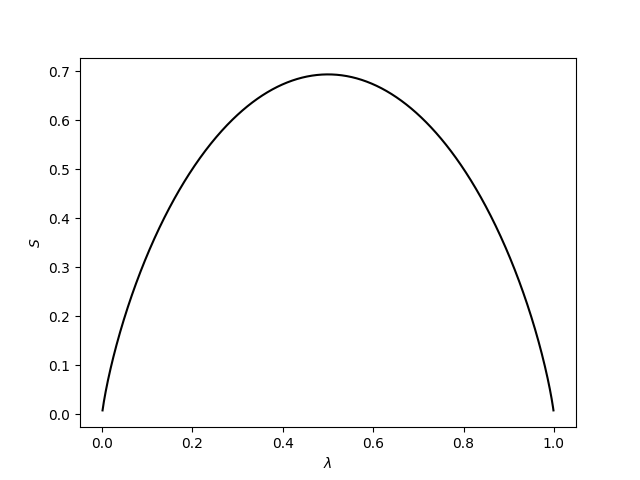
\includegraphics[width=0.8\textwidth]{entropia_M2.png}
\caption{The entropy of equation \ref{eq:entropy_M2} as a function of the probability that the photon has horizontal polarization.}
\end{figure}
\end{example}

For completeness we state a theorem given by \cite{Bratteli1997} that shows that every GNS representation can be decomposed into representations with a cyclic vector.

\begin{theorem}
Every non-degenerate representation $(\mathcal{H},\pi)$ of a $C^*$-algebra $\mathcal{A}$ (that is, one in which $\pi(\mathcal{A})x={0}$ implies $x=0$) is a direct sum of representations with a cyclic vector. 
\end{theorem}

\section{Von Neumann Algebras}

In this section we will explore the theory of von Neumann algebras. Although these are special cases of $C^*$-algebras, they will be the correct setting to develop Tomita-Takesaki theory and eventually connect it with KMS states. Moreover, their study is also important for the general theory of quantum systems with infinite degrees of freedom including quantum field theories\cite{Haag1992}. In this case, to be concrete we will follow the presentation of \cite{ Evans1998}. 

\begin{definition}
Let $\mathfrak{M}\subseteq \mathcal{B}({\mathcal{H}})$ for some Hilbert space $\mathcal{H}$. The commutant of $\mathfrak{M}$ is
\begin{equation}
\mathfrak{M}'=\{A\in\mathcal{B}(\mathcal{H})|AB=BA\text{ for all } B\in\mathfrak{M}\}.
\end{equation}
We say $\mathfrak{M}$ is a von Neumann algebra ($W^*$-algebra) if $\mathfrak{M}''=\mathfrak{M}$.
\end{definition}

\begin{example}
It is clear that for all $\mathfrak{M}\subseteq\mathcal{B}(\mathcal{H})$ for some Hilbert space $\mathcal{H}$ we have $\mathfrak{M}\subseteq\mathfrak{M}''$. Therefore $\mathcal{B}(\mathcal{H})$ is a $W^*$-algebra.
\end{example}

We claimed that every $W^*$-algebras is a $C^*$-algebra. Indeed,

\begin{theorem}
Let $\mathfrak{M}\subseteq \mathcal{B}({\mathcal{H}})$ for some Hilbert space $\mathcal{H}$ be self-adjoint. Then $\mathfrak{M}'$ is a $C^*$-algebra.
\end{theorem}

\begin{proof}
It is a matter of checking that $\mathfrak{M}'$ is a *-algebra. It is clear that for all $A\in\mathfrak{M}'$ we have $\|A^*A\|=\|A\|^2$ since this is true in $\mathcal{B}(\mathcal{H})$. Finally, if $(A_n)$ is a Cauchy sequence in $\mathfrak{M}'$ then it converges to some $A\in\mathcal{B}(\mathcal{H})$. Since multiplication is continuous (a simple consequence of the compatibility between multiplication and the norm in $C^*$-algebras and therefore in $\mathcal{B}(\mathcal{H})$) we have that
\begin{align}
\begin{split}
AC&=(\lim_{n\rightarrow\infty}A_n)C = \lim_{n\rightarrow\infty}A_nC=\lim_{n\rightarrow\infty}CA_n \\
&= C\lim_{n\rightarrow\infty}A_n=CA.
\end{split}
\end{align}
Therefore $\mathfrak{M}'$ is Banach and we conclude it is a $C^*$-algebra.
\end{proof}

\begin{corollary}\label{cor:W_C}
A $W^*$-algebra is a $C^*$-algebra.
\end{corollary}

\begin{theorem}
Let $\mathfrak{M}$ be a von Neumann algebra on a Hilbert space $\mathcal{H}$ and $G\subseteq\mathcal{H}$. Then $G$ is cyclic for $\mathfrak{M}$ if and only if $G$ is separating for $\mathfrak{M}'$.
\end{theorem}

\begin{proof}
Suppose $G$ is cyclic for $\mathfrak{M}$ and let $A\in\mathcal{M}'$ be such that $AG=\{0\}$. Then for all $\mathcal{B}\in\mathfrak{M}$ and $x\in G$ we have $ABx=BAx=B0=0$. By continuity $A=0$.
Conversely, suppose $G$ is separating for $\mathfrak{M}'$ and let $P$ be the orthogonal projection on $\overline{\mathfrak{M}G}$. We will prove that the projection onto its orthogonal complement is null. First note that $P\in\mathfrak{M}'$. Indeed, if $x\in\mathcal{H}$ there exists $y\in \overline{\mathfrak{M}G}$ and $z\in\overline{\mathfrak{m}G}^\bot$ such that $x=y+z$. If $A\in\mathfrak{M}$ then $Ay\in\overline{\mathfrak{M}G}$ and $APy=Ay=PAy$. On the other hand, $Az\in\overline{\mathfrak{m}G}^\bot$ since for all $v\in\overline{\mathfrak{m}G}$ we have $\langle v,Az\rangle=\langle A^*v,z\rangle=0$. Therefore $PAz=0=A0=APz$. We conclude that $PAx=APx$ and $P\in\mathfrak{M}'$.Then it is clear that $1-P\in\mathfrak{M}'$ and we have $(1-P)G=\{0\}$. Since $G$ is separating for $\mathfrak{M}'$ we have $1-P=0$ and therefore $P=1$ showing that $G$ is cyclic for $\mathfrak{M}$.
\end{proof}

As it turns out, the GNS representation of a von Neumann algebra equipped with a faithful normal state will have properties which as we will see later are suitable for the application of Tomita-Takesaki theory.

\begin{theorem}\label{thm:GNS_von}
Let $\mathfrak{M}$ be a $W^*$-algebra and $\omega$ be a normal faithful state. Then the GNS representation $(\mathcal{H}_\omega,\pi_\omega)$ is faithful, $\pi_\omega(\mathfrak{M})$ is a $W^*$-algebra and the cyclic vector $\Omega_\omega$ is separating for $\pi_\omega(\mathfrak{M})$.
\end{theorem} 

\begin{proof}
The fact that $\pi_\omega(\mathfrak{M})$ is a $W^*$-algebra is given in \cite{Bratteli1997} and relies on the topological properties of von Neumann algebras which we have not discussed. Let $A\in\mathfrak{M}$ be such that $\pi_\omega(A)\Omega_\omega=0$ (which in particular is true if $A\in\ker\pi_\omega$). Then since $\omega$ is faithful and
\begin{equation}
\omega(A^*A)=\langle \Omega_\omega, \pi_\omega (A^*A)\Omega_\omega\rangle=\langle \pi_\omega(A)\Omega_\omega,\pi_\omega(A)\Omega_\omega\rangle=0
\end{equation}
we conclude that $A^*A=0$. Therefore by the $C^*$-property $0=\|A^*A\|=\|A\|^2$ and $A=0$. We conclude that the representation is faithful and $\Omega_\omega$ is separating for $\pi_\omega(\mathfrak{M})$.
\end{proof}

\section{Dynamical Systems}

Up until now, we have only focused on the description of observables and states of a physical system. In now way have we yet discussed the dynamics of a system. In the context of algebraic physics we have that the concept of time evolution is implemented through automorphisms of the algebra of observables. To show this we will follow \cite{Duvenhage1999}.

\begin{definition}\label{def:dynamics}
Let $\mathcal{A}$ be a $C^*$-algebra. A one-parameter automorphism group is a group homomorphism $\tau:\mathbb{R}\rightarrow \Aut(\mathcal{A})$ $t\mapsto\tau_t$. If $\tau$ is a one-parameter automorphism group where the map $\mathbb{R}\rightarrow\mathcal{A}$ given by $t\mapsto\tau_t(A)$ is continuous for all $A\in\mathcal{A}$, then $(\mathcal{A},\tau)$ is called a $C^*$-dynamical system. If $\mathfrak{M}$ is a $W^*$-algebra on a Hilbert space $\mathcal{H}$ and $\tau$ is a one-parameter automorphism group on $\mathfrak{M}$ such that $\mathbb{R}\rightarrow\mathcal{H}$ given by $t\mapsto\tau_t(A)x$ is continuous for all $A\in\mathfrak{M}$ and $x\in\mathcal{H}$, then $(\mathfrak{M},\tau)$ is called a $W^*$-dynamical system. 
\end{definition}

The distinction we make for von Neumann algebras reflects the fact that even though we have corollary \ref{cor:W_C}, von Neumann algebras will be more general in physical applications. Indeed we have,

\begin{theorem}\label{thm:C_W}
A $C^*$-dynamical system whose underlying algebra is a $W^*$-algebra is a $W^*$-dynamical system.
\end{theorem}

\begin{proof}
Let $\mathfrak{M}$ be a $W^*$-algebra on a Hilbert space $\mathcal{H}$ and $(\mathfrak{M},\tau)$ a $C^*$-dynamical system. Notice that for every $x\in\mathcal{H}$ the evaluation map $\ev_{x}:\mathfrak{M}\rightarrow \mathcal{H}$ given by $\ev_{x}(A)=Ax$ is continuous. Indeed if $\epsilon\in\mathbb{R}^+$, $\delta=\epsilon/\|x\|$, and $\|A-B\|<\delta$ for $A,B\in\mathfrak{M}$ then
\begin{equation}
\|Ax-Bx\|=\|(A-B)x\|\leq\|A-B\|\|x\|<\frac{\epsilon}{\|x\|}\|x\|=\epsilon.
\end{equation}
Then the map $\mathbb{R}\rightarrow\mathcal{H}$ $t\mapsto\tau_t(A)x$, being $\ev_{x}$ after $\mathbb{R}\rightarrow\mathcal{A}$ $t\mapsto\tau_t(A)$ continuous by hypotheses, is continuous for all $A\in\mathfrak{M}$ and $x\in\mathcal{H}$. The conclusion follows.
\end{proof}

Following \cite{Duvenhage1999} we will from now on restrict to finite dimensional Hilbert spaces to inspire notions which we will however generalize later by using definition \ref{def:dynamics}.

\begin{example}\label{ex:schrodinger}
In quantum mechanics we already have a dynamical law given by Schrödinger's equation. Consider a finite dimensional Hilbert space $\mathcal{H}$ with a self-adjoint Hamiltonian $H$. The time evolution, as prescribed by Heisenberg's representation of Schrodinger's mechanics is the restriction of
\begin{alignat}{2}
\tau:\mathbb{C}&\rightarrow&\Aut(\mathcal{B}(\mathcal{H})) \nonumber \\
z&\mapsto&\tau_z:\mathcal{B}(\mathcal{H})&\rightarrow\mathcal{B}(\mathcal{H}) \\
&&A&\mapsto e^{iHz}Ae^{-iHz} \nonumber
\end{alignat}
to the real numbers. The verification that this map is well defined and indeed restricts to a one-parameter automorphism group is routine.
Let $\{e_1,\dots,e_N\}$ be an orthonormal basis of eigenvectors of $H$ associated to the eigenvalues $E_1,\dots,E_N$ (whose existence is guaranteed by the spectral theorem). Then we have
\begin{align}
\begin{split}
\|e^{iHt}-1\|&=\|\sum_{n=1}^Ne^{iE_nt}\rho_{e_n}-\sum_{n=1}^N \rho_{e_n}\|\leq\sum_{n=1}^N \|\left(e^{iE_nt}-1\right)\rho_{e_n}\| \\
&= \sum_{n=1}^N|e^{iE_nt}-1|\|\rho_{e_n}\|=\sum_{n=1}^N|e^{iE_nt}-1|\rightarrow 0
\end{split}
\end{align}
as $t\rightarrow 0$. Therefore if $s\in\mathbb{R}$ we have
\begin{align}
\begin{split}
\lim_{t\rightarrow s}\tau_t(A)=\lim_{t\rightarrow s}\tau_{t-s}\tau_s(A)=\lim_{t\rightarrow s}e^{iH(t-s)}\tau_s(A)e^{iH(s-t)}=\tau_s(A)
\end{split}
\end{align}
for all $A\in \mathcal{B}(\mathcal{H})$. We conclude that $(\mathcal{B}(\mathcal{H}),\tau)$ is a $C^*$ and $W^*$-dynamical system.
\end{example} 

Note that even though the dynamics have been defined through automorphisms of the algebra resembling Heisenberg's quantum mechanics, we could've equally defined it analogously to Schrodinger's mechanics through the evolution of states
\begin{equation}
\tau_t(\omega)(A):=\omega(\tau_t(A)).
\end{equation}
This is of course yields the same physics and we will occasionally use it to give a physical interpretation to mathematical results. 

The following consequence given in \cite{Duvenhage1999} of having a state invariant under the dynamics of a system for its GNS representation will be useful later on to formulate the connection between KMS states and Tomita-Takesaki theory.

\begin{theorem}
Let $\mathcal{A}$ be a $C^*$-algebra, $\tau$ a one-parameter group of automorphisms of $\mathcal{A}$, $\omega$ a state such that $\omega(\tau_t(A))=\omega(A)$ for all $t\in\mathbb{R}$ and $A\in\mathcal{A}$, and $(\mathcal{H}_\omega,\pi_\omega)$ the induced GNS representation. Then there exists a unique one-parameter unitary group
\begin{align}
\begin{split}
U:\mathbb{R}&\rightarrow\{A\in\mathcal{B}(\mathcal{H})|A\text{ is unitary}\} \\
t&\mapsto U_t
\end{split}
\end{align}
such that $U_t\Omega_\omega=\Omega_\omega$ and $\pi_\omega(\tau_t(A))=U_t\pi_\omega(A)U_{-t}$ for all $t\in\mathbb{R}$ and $A\in\mathcal{A}$. Furthermore, if $(\mathcal{A},\tau)$ is a $W^*$-dynamical system and $\pi_\omega(\mathcal{A}$ is a von Neumann algebra, then $U$ is strongly continuous.
\end{theorem} 

\begin{proof}
Notice that $(\mathcal{H}_\omega,\pi\circ\tau_t)$ is a representation for all $t\in\mathbb{R}$ which satisfies the properties of the GNS representation, namely, $\Omega_\omega$ is cyclic. Then, by uniqueness, we have the unique desired function $U$. We only need to show $U$ is a group homomorphism. 
\end{proof}

\bibliography{Monografia}

\end{document}